% Workshop wiskunde,  Jeroen Zuiddam

% beamer
\documentclass{beamer}
\mode<presentation>

% packages
\usepackage{amsmath,amssymb, amsfonts,mathrsfs}
\usepackage[dutch]{babel}
%\usepackage{hyperref}
\usepackage{graphicx}
%\usepackage{tikz}
%\usepackage{pgfplots}
%\usetikzlibrary{arrows}
%\usetikzlibrary{positioning}
%\usepackage{stmaryrd}
\usetheme{Watergraafsmeer}

\usepackage{enumerate}

% For every picture that defines or uses external nodes, you'll have to
% apply the 'remember picture' style. To avoid some typing, we'll apply
% the style to all pictures.
%\tikzstyle{every picture}+=[remember picture]

% front stuff
\author{Joris Stork en Jeroen Zuiddam}
\title{Kinect: hoe werkt het?}
\date{}

\begin{document}

%% frame %%
\setbeamercolor{headline}{parent=white}
\begin{frame}
\titlepage
\end{frame}
\setbeamercolor*{headline}{parent=palette primary}
\section{}

\begin{frame}{Kinect}{}
\centerline{
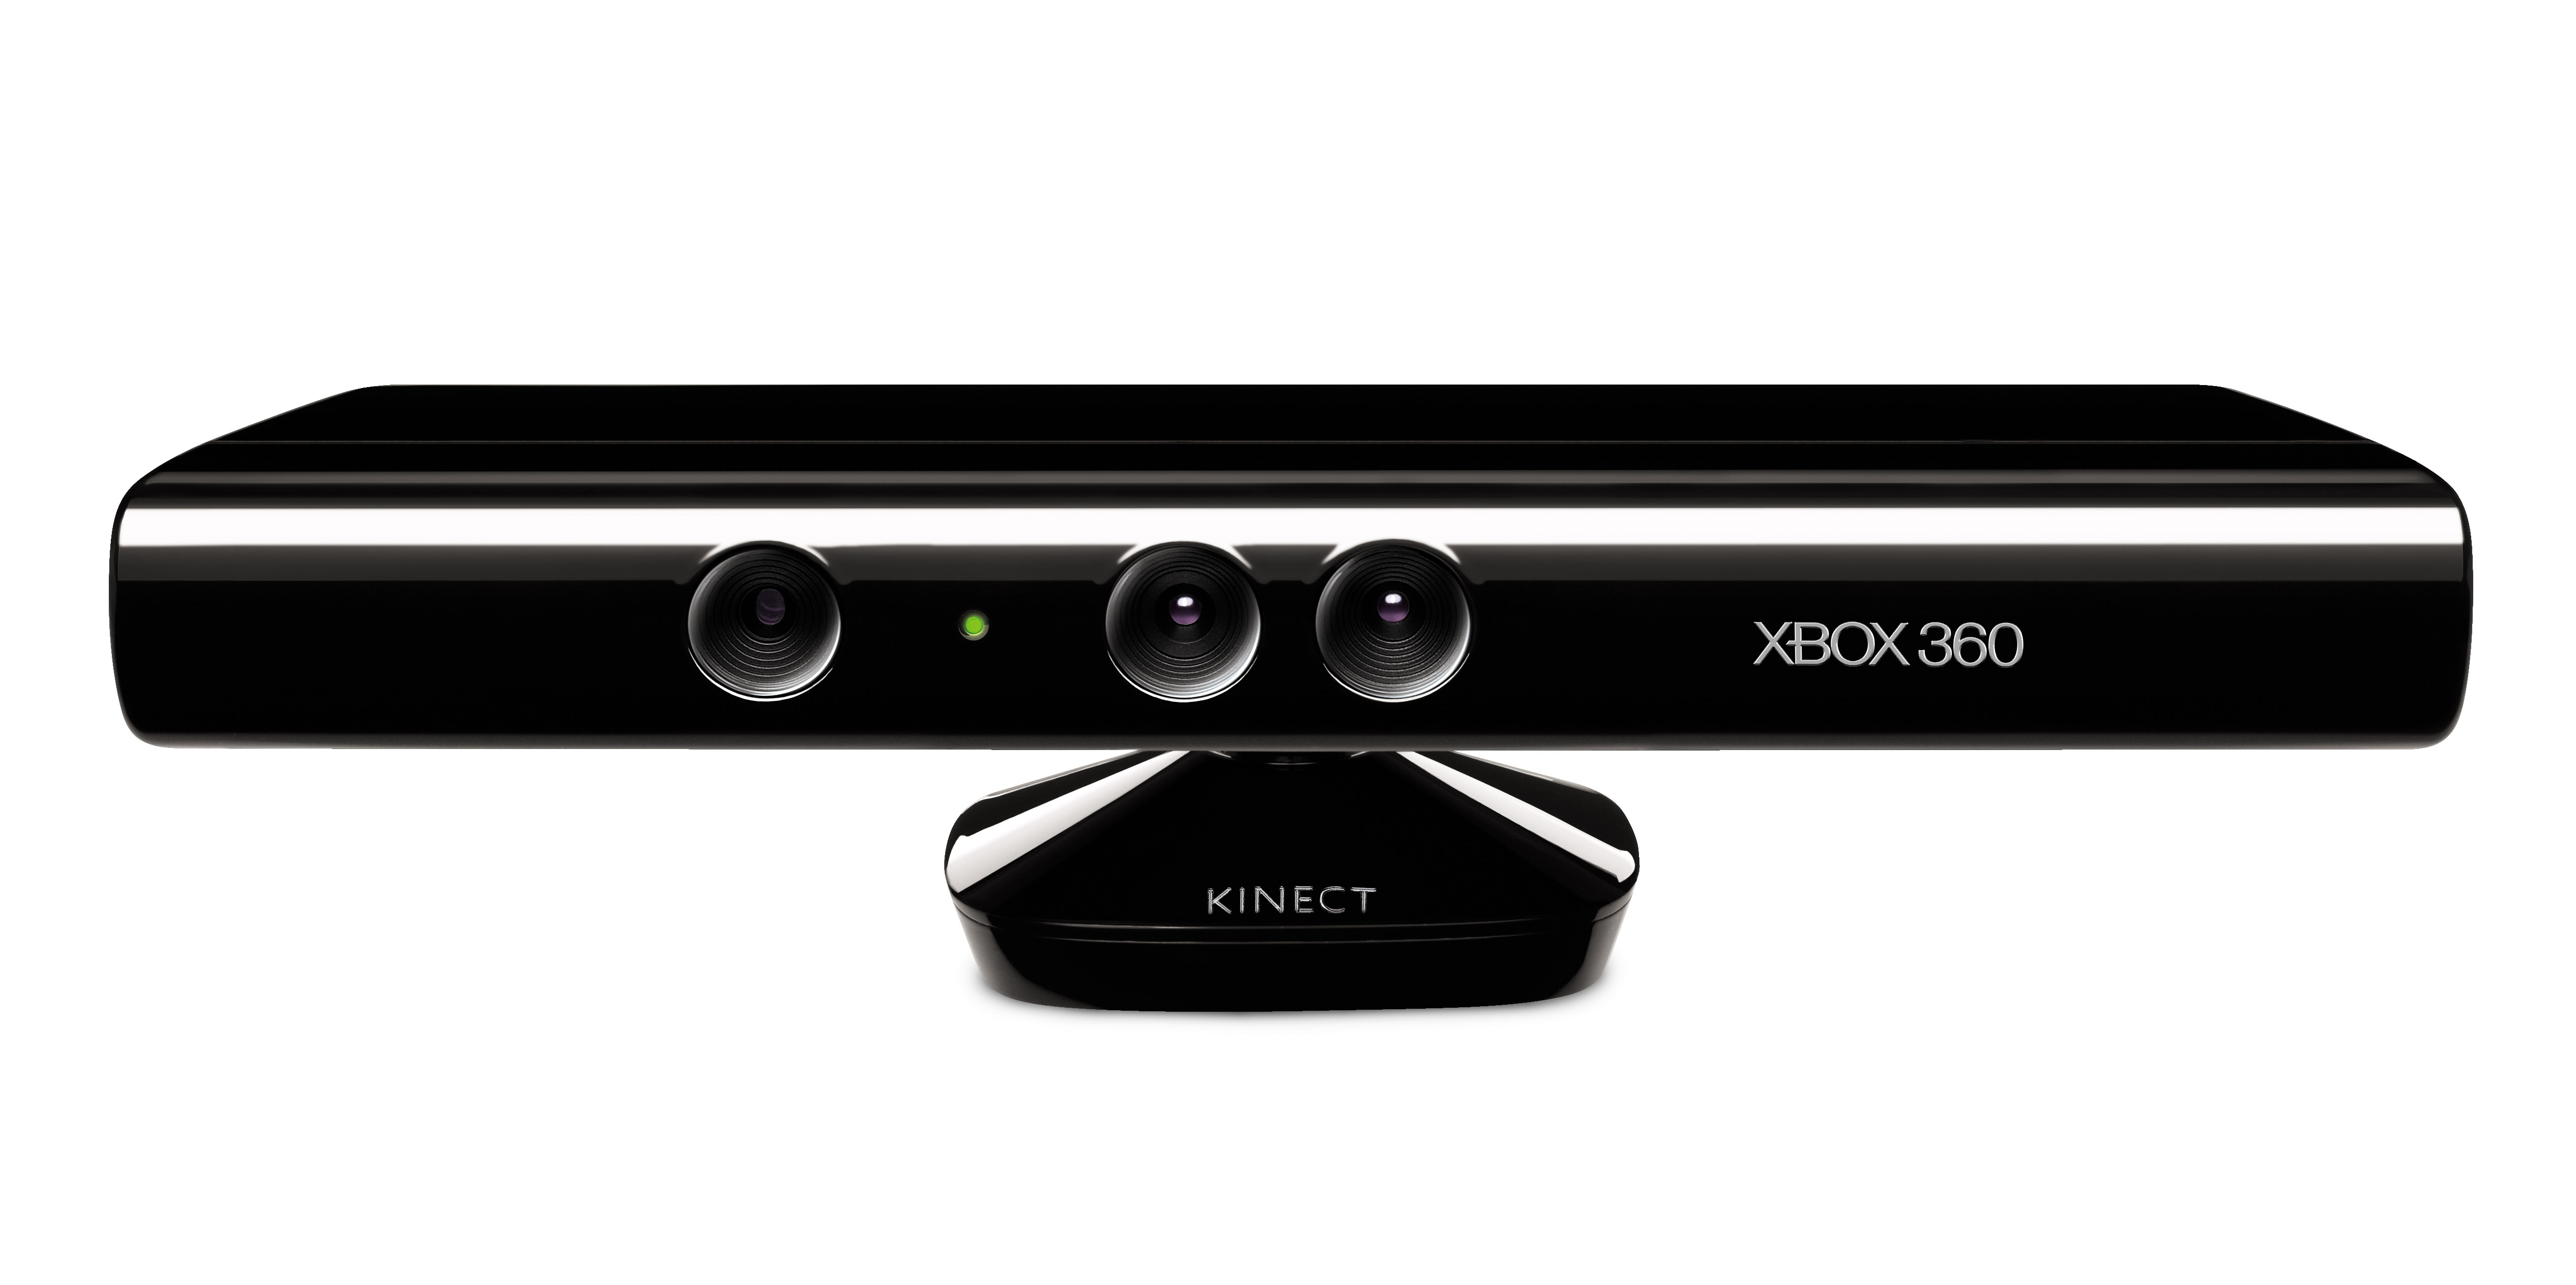
\includegraphics[scale=0.3, viewport= 40 120 1190 460, clip=true]{kinect.jpg}
}

\pause
\vfill
\begin{columns}
\column{.25\textwidth}
project:
\begin{enumerate}
\item \alt<3->{\textbf{werking}}{werking}
\item applicatie
\end{enumerate}
\pause
\column{.5\textwidth}
vandaag:
\begin{enumerate}
\item stereotriangulatie
\item correspondence problem
\end{enumerate}
\end{columns}
\end{frame}

\begin{frame}{Stereotriangulatie}

{\large Algemene situatie: twee willekeurige camera's}

\centerline{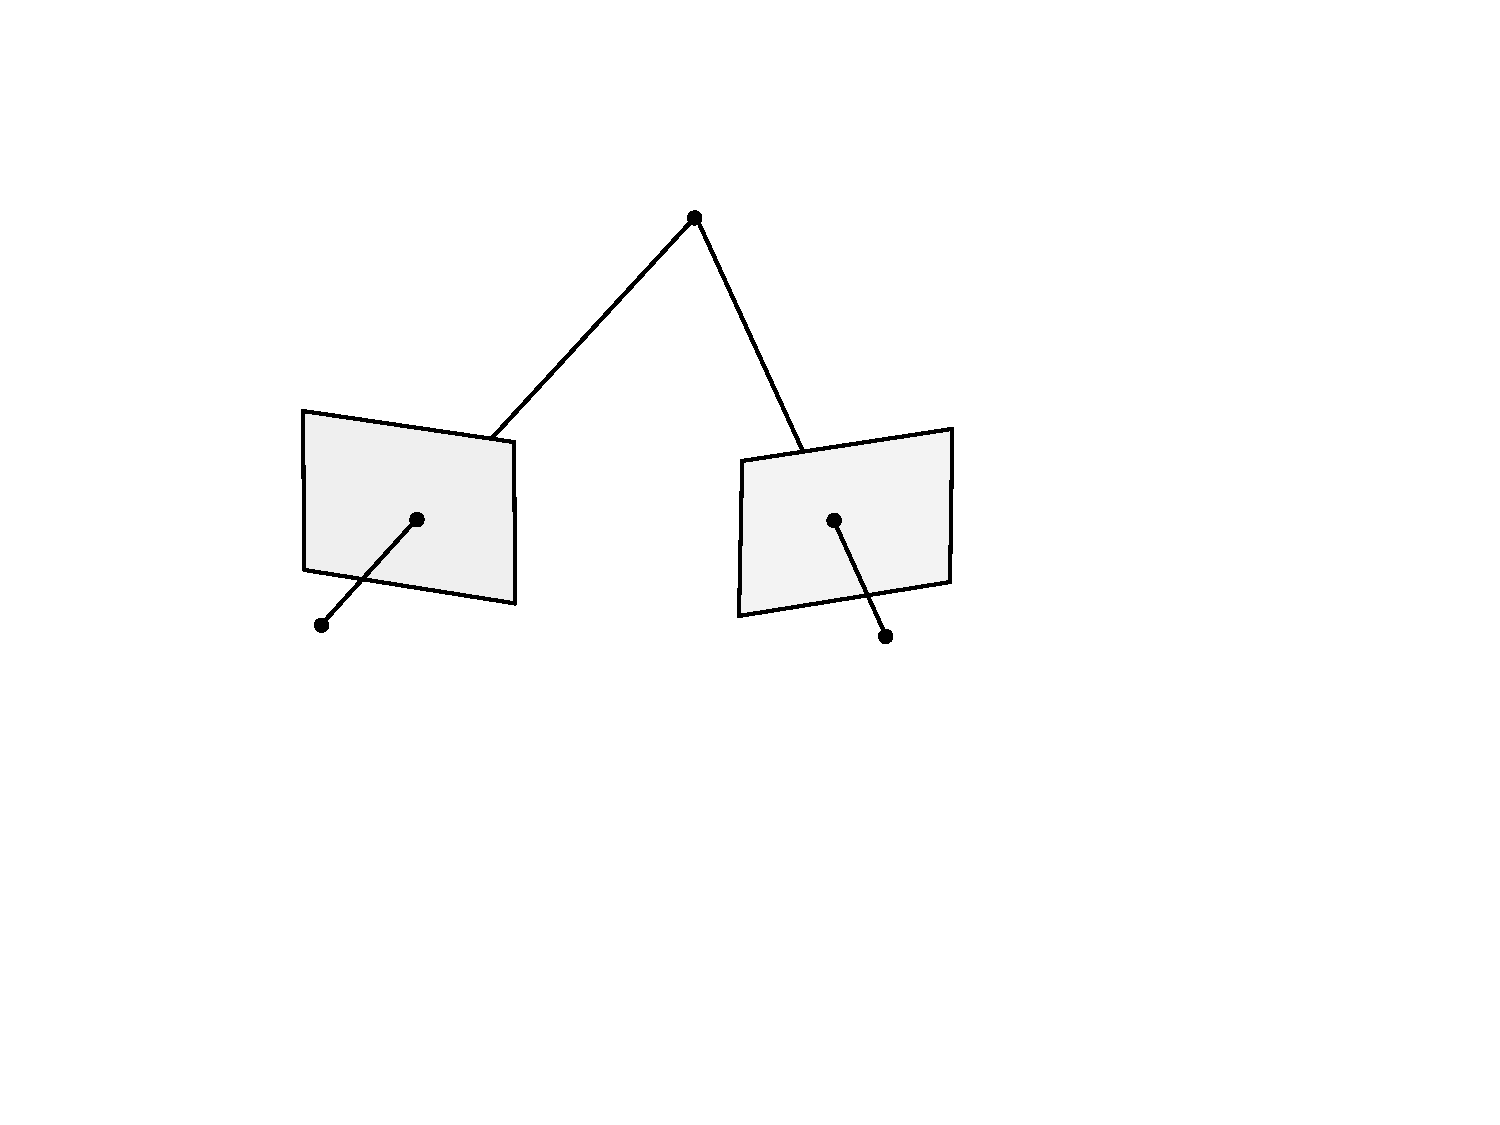
\includegraphics[scale=0.4, clip=true, viewport= 120 230 470 470]{triang}}
\vfill
\pause
{\large Rekenvoorbeeld: twee parallele pinhole cameras}
\pause
$$
\frac{z_1}{b} = \frac{z_1 - f}{b-x_l+x_r}\quad \pause\implies\quad z_1 = \frac {bf} {x_l - x_r}
$$
\end{frame}

\begin{frame}{Actieve stereotriangulatie}{}
{\large Algemene situatie}
\begin{enumerate}
\item camera
\item projector, laser of lamp
\end{enumerate}
\vfill
\pause
\centerline{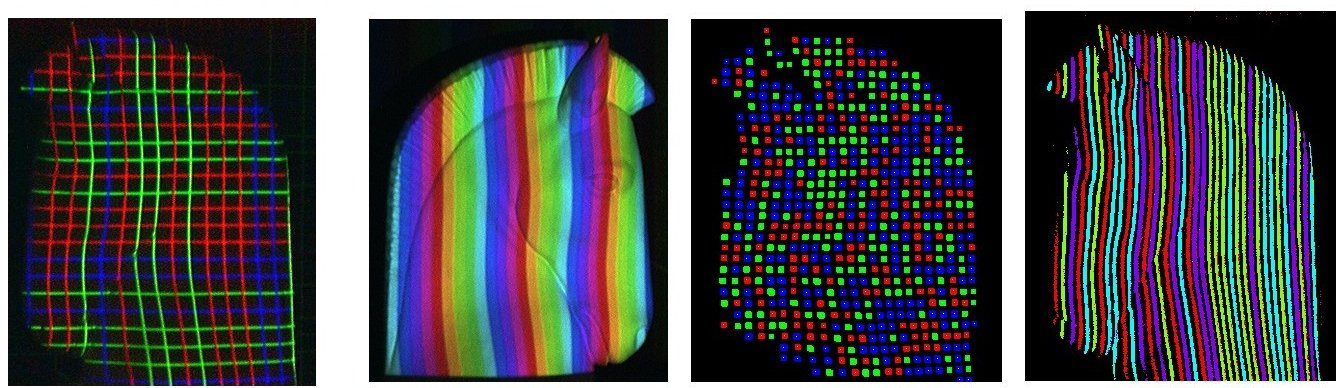
\includegraphics[scale=0.17]{structuredlight.jpg}\, 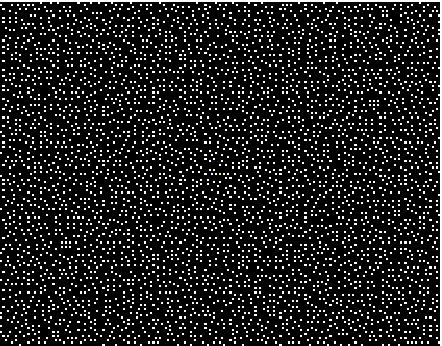
\includegraphics[scale=1, clip=true, viewport= 0 0 80 63]{kinect-pattern}}
\vfill
\pause
{\large Rekenvoorbeeld: `Kinect' met \'e\'en geprojecteerd punt}
\pause
$$
z_1 = \frac {z_0bf}{bf + r_0d}
$$
\end{frame}

\begin{frame}{Actieve stereotriangulatie}\vspace{-4pt}
\centerline{\includegraphics[scale=0.15, viewport=50 0 2700 1800, clip=true]{kinect_speckle.jpg}}
\end{frame}

%\begin{frame}{Actieve stereotriangulatie}\vspace{-4pt}
%\centerline{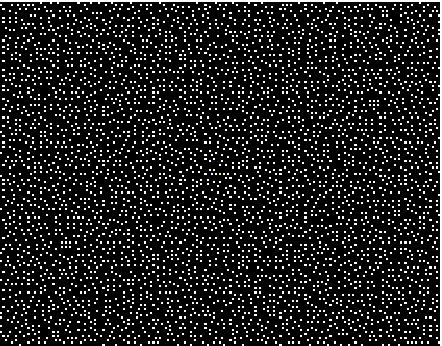
\includegraphics[scale=1.3]{kinect-pattern}}
%\end{frame}

\begin{frame}{Correspondence problem}

\begin{block}{Correspondence problem}
Welke referentiepunt hoort bij mijn punt?
\end{block}
\vfill
\pause
{\large Een oplossing}
\begin{columns}[t]
\column{.6\textwidth}
\begin{enumerate}
\item<+-> maak referentiebeelden
\item<+-> neem camerabeeld
\item<+-> voor elk punt
\begin{enumerate}[a.]
\item<+-> neem regio
\item<+-> bepaal schaal
\item<+-> correleer regio over referentiebeeld met die schaal
\item<+-> punt met hoogste correlatie is referentiepunt
\end{enumerate}
\end{enumerate}
\column{.4\textwidth}
\uncover<2->{ref.\\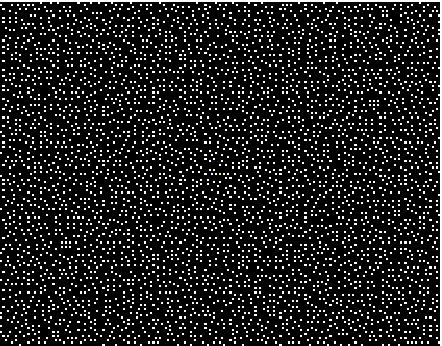
\includegraphics[scale=0.4]{kinect-pattern}}
\\
\uncover<3->{camera\\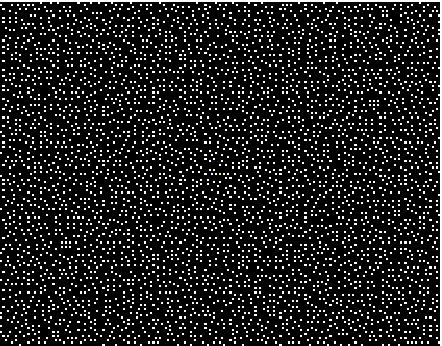
\includegraphics[scale=0.4]{kinect-pattern}}
\end{columns}
\end{frame}

\setbeamercolor{headline}{parent=white}
\begin{frame}

\end{frame}
\setbeamercolor*{headline}{parent=palette primary}
\section{}

\end{document}
